\documentclass[a4paper, 11pt, twoside]{article}

%\usepackage[ngerman]{babel}
\usepackage[english]{babel}
\usepackage[latin1]{inputenc}

\usepackage{graphicx,float}
%\usepackage{pifont}
\usepackage{type1cm}
\usepackage{amssymb, amsthm, amsmath}
\usepackage{listings}
\usepackage{pgf}
\usepackage{url}
\usepackage{hyperref}

\usepackage{makeidx}
\makeindex

\setlength{\parindent}{0em}
\setlength{\oddsidemargin}{0.0cm}
\setlength{\evensidemargin}{0.0cm}
\setlength{\textheight}{24.0cm}
\setlength{\topmargin}{-1.0cm}
\setlength{\footskip}{1.5cm}
\setlength{\textwidth}{15.5cm}

\renewcommand*\familydefault{\sfdefault}
\newcommand{\dd}{\mathrm{d}}
\newtheorem{problem}{Problem}[section]
\newtheorem{theorem}{Theorem}[section]
\newtheorem{remark}{Remark}[section]

\begin{document}
\pagestyle{empty}
%\documentclass[a4paper]{article}

%\usepackage{pgf}
%\usepackage{graphicx}
%\usepackage{pifont}
%\usepackage{type1cm}

\setlength{\textwidth}{14cm}
\setlength{\oddsidemargin}{1cm}

%\begin{document}

\pagestyle{empty}

%%%%%%%%%%%%%%%%%%%%%%%%%%%%%%%%%%%%%%%%
%%%%%%%%%%%%%%%%%%%%%%%%%%%%%%%%%%%%%%%%
%%%%%%%%%%%%%%%%%%%%%%%%%%%%%%%%%%%%%%%%

\newcount \Z
\Z=20

%%% logos %%%

%%% NUMHPC %%%
\newlength{\numhpclogox}
\setlength{\numhpclogox}{\paperwidth} % 20/210ths of the paperwidth
\divide\numhpclogox by 210
\multiply\numhpclogox by 100

\newlength{\numhpclogoy}
\setlength{\numhpclogoy}{\paperheight} % 270/297ths of the paperwidth
\divide \numhpclogoy by 297
\multiply \numhpclogoy by -235

\newlength{\numhpclogoheight}
\setlength{\numhpclogoheight}{\paperheight} % 270/297ths of the paperwidth
\divide\numhpclogoheight by 297
\multiply\numhpclogoheight by 20

%%% KIT %%%
\newlength{\kitlogox}
\setlength{\kitlogox}{\paperwidth} % 20/210ths of the paperwidth
\divide\kitlogox by 210
\multiply\kitlogox by 0

\newlength{\kitlogoy}
\setlength{\kitlogoy}{\paperheight} % 270/297ths of the paperwidth
\divide \kitlogoy by 297
\multiply \kitlogoy by -230

\newlength{\kitlogoheight}
\setlength{\kitlogoheight}{\paperheight} % 270/297ths of the paperwidth
\divide\kitlogoheight by 297
\multiply\kitlogoheight by 15


%%% EMCL %%%
\newlength{\emcllogox}
\setlength{\emcllogox}{\paperwidth} % 20/210ths of the paperwidth
\divide\emcllogox by 210
\multiply\emcllogox by 28

\newlength{\emcllogoy}
\setlength{\emcllogoy}{\paperheight} % 270/297ths of the paperwidth
\divide \emcllogoy by 297
\multiply \emcllogoy by -160

\newlength{\emcllogoheight}
\setlength{\emcllogoheight}{\paperheight} % 270/297ths of the paperwidth
\divide\emcllogoheight by 297
\multiply\emcllogoheight by 20

%%% HIFLOW %%%
\newlength{\hiflowlogox}
\setlength{\hiflowlogox}{\paperwidth} % 20/210ths of the paperwidth
\divide\hiflowlogox by 210
\multiply\hiflowlogox by 28

\newlength{\hiflowlogoy}
\setlength{\hiflowlogoy}{\paperheight} % 270/297ths of the paperwidth
\divide \hiflowlogoy by 297
\multiply \hiflowlogoy by -160

\newlength{\hiflowlogoheight}
\setlength{\hiflowlogoheight}{\paperheight} % 270/297ths of the paperwidth
\divide\hiflowlogoheight by 297
\multiply\hiflowlogoheight by 33

%%%%%%%%%%%%%%%%%%%%%%%%%%%%%%%%%%%%%%%%
%%%%%%%%%%%%%%%%%%%%%%%%%%%%%%%%%%%%%%%%
%%%%%%%%%%%%%%%%%%%%%%%%%%%%%%%%%%%%%%%%

%%% NUMHPC %%%
%%\pgftext[bottom, left, at={\pgfpointadd{\pgfpoint{0pt}{0pt}}{\pgfpoint{\numhpclogox}{\numhpclogoy}}}]{\includegraphics[totalheight=\numhpclogoheight]{numhpc}}

%%% KIT %%%
%%\pgftext[bottom, left, at={\pgfpointadd{\pgfpoint{0pt}{0pt}}{\pgfpoint{\kitlogox}{\kitlogoy}}}]{\includegraphics[totalheight=\kitlogoheight]{kitlogo}}

%%% EMCL %%%
\pgftext[bottom, left, at={\pgfpointadd{\pgfpoint{0pt}{0pt}}{\pgfpoint{\hiflowlogox}{\hiflowlogoy}}}]{
\includegraphics[totalheight=\hiflowlogoheight]{HF3_color}}

%%% horizontal lines %%%
\pgfline{\pgfxy(-1pt,0.1pt)}{\pgfxy(15pt,0.1pt)}
\pgfline{\pgfxy(-1pt,-21.4pt)}{\pgfxy(15pt,-21.4pt)}
%%\pgfline{\pgfxy(-1pt,-22.4pt)}{\pgfxy(15pt,-22.4pt)}

%%% EMCL text %%%
\pgftext[bottom, left, at={\pgfpointadd{\pgfpoint{0pt}{0pt}}{\pgfpoint{0cm}{1cm}}}]{{\LARGE{{\bf Tutorial}}}}

%%% EMCL web %%%
\pgftext[bottom, left, at={\pgfpointadd{\pgfpoint{0pt}{0pt}}{\pgfpoint{10.5cm}{-21.7cm}}}]{{\fontsize{13}{10}\selectfont{} http://www.hiflow3.org/}}

\hspace{2cm}
\begin{picture}(0,0)(-250,-25)

\includegraphics[scale=.22]{emcl.pdf} 
\end{picture}

%%% author %%%
\pgftext[bottom, left, at={\pgfpointadd{\pgfpoint{0pt}{0pt}}{\pgfpoint{0cm}{-4cm}}}]{{
\begin{parbox}{13cm}{
\begin{center}\fontsize{12}{30}\selectfont{} C. Straub, S. Gawlok
\end{center}}
\end{parbox}}}

%%% title %%%
\pgftext[bottom, left, at={\pgfpointadd{\pgfpoint{0pt}{0pt}}{\pgfpoint{0cm}{-7.5cm}}}]{{
\begin{parbox}{13cm}{
%%\begin{center}\fontsize{18}{30}\selectfont{} \bf Using HiFlow$^3$ for solving the
\begin{center}\fontsize{22}{30}\selectfont{} \bf Stabilization Schemes for Advection Dominated Stationary Convection-Diffusion Equation
\end{center}}
\end{parbox}}}

%%% date %%%
\pgftext[bottom, left, at={\pgfpointadd{\pgfpoint{0pt}{0pt}}{\pgfpoint{0cm}{-16.4cm}}}]{{
\begin{parbox}{13cm}{
\begin{center}\fontsize{12}{24}\selectfont{}
\vspace{5cm}
\textit{modified on \today}\\
\vspace{6.5cm}
\hspace{6cm}\textit{Version 1.3}
\end{center}}
\end{parbox}}}

%fhfh \hfill sjdh

%\end{document}


%\newpage
%\null\newpage

\tableofcontents

\newpage
\pagestyle{plain}
\framebox[15.5cm]{\parbox[c][2.3cm]{14.5cm}{
\fontsize{19}{19}\selectfont{} \bf{Time-Discretization Methods Based on Convection-Diffusion Equation}
}}
\vspace{0.5cm}
\section{Introduction}

HiFlow$^3$ is a multi-purpose finite element software providing powerful tools for efficient and accurate solution of a wide range of problems modeled by partial differential equations (PDEs). Based on object-oriented concepts and the full capabilities of C++ the HiFlow$^3$ project follows a modular and generic approach for building efficient parallel numerical solvers. It provides highly capable modules dealing with the mesh setup, finite element spaces, degrees of freedom, linear algebra routines, numerical solvers, and output data for visualization. Parallelism - as the basis for high performance simulations on modern computing systems - is introduced on two levels: coarse-grained parallelism by means of distributed grids and distributed data structures, and fine-grained parallelism by means of platform-optimized linear algebra back-ends.

\subsection{How to Use the Tutorial?}
You find the example code (instationary\_convdiff\_tutorial.cc, instationary\_convdiff\_tutorial.h), a parameter file for the first numerical example (instationary\_convdiff\_tutorial.xml) and a Makefile, which you only need when using HiFlow$^3$ as a library (see \ref{sectionlibrary}), in the folder \newline \verb'/hiflow/examples/convection_diffusion'. The geometry data (*.inp, *.vtu) is stored in the folder \verb'/hiflow/examples/data'.

\subsubsection{Using HiFlow$^3$ as a Library}\label{sectionlibrary}
First install HiFlow$^3$. Therefore, follow the instructions listed on \verb'http://www.hiflow3.org/', see "Documentation"-"Installation".
To compile and link the tutorial correctly, you may have to adapt the Makefile depending on the options you chose in the cmake set up. Make sure that the variable \verb'HIFLOW_DIR' is set to the path, where HiFlow$^3$ was installed. The default value ist \verb'/usr/local'. When you set the option \verb'WITH_METIS' to \verb'ON' in the cmake set up, you have to make sure to link to the metis library in the Makefile (\url{www.cs.umn.edu/~metis}). \texttt{-lmetis} must be added to the end of the line in the Makefile, where the target 
\texttt{instationary\_convdiff\_tutorial} is build (see second option in the Makefile, which is marked as a comment). By typing \verb'make' in the console, in the same folder where the source-code and the Makefile is stored, you compile and link the tutorial. 
To execute the instationary convection-diffusion tutorial sequentially, type \textbf{./instationary\_convdiff\_tutorial} \verb'/"path_to"/instationary_convdiff_tutorial.xml' \verb'/"path_to_mesh_data"/' . To execute it in parallel mode \index{program!executing in parallel} with four processes type \newline \textbf{mpirun -np 4 ./instationary\_convdiff\_tutorial} \verb'/"path_to"/instationary_convdiff_tutorial.xml' \verb'/"path_to_mesh_data"/' .

\subsubsection{Using HiFlow$^3$ as a Developer}\label{sectiondeveloper}
First build and compile HiFlow$^3$. Go to the directory \verb'/build/example/convection_diffusion', where the binary \textbf{instationary\_convdiff\_tutorial} is stored. Type \textbf{./instationary\_convdiff\_tutorial}, to execute the program in sequential mode. To execute in parallel mode \index{program!executing in parallel} with four processes, type \textbf{mpirun -np 4 ./instationary\_convdiff\_tutorial}. In both cases, you need to make sure that the default parameter file instationary\_convdiff\_tutorial.xml is stored in the same directory as the binary, and that the geometry data specified in the parameter file is stored in \verb'/hiflow/examples/data'. Alternatively, you can specify the path of your own xml-file with the name of your xml-file (first) and the path of your geometry data (second) in the comment line, i.e. \newline \textbf{./instationary\_convdiff\_tutorial} \verb'/"path_to_parameterfile"/"name_of_parameterfile".xml'
\verb'/"path_to_geometry_data"/'.

\section{Mathematical Setup}
\subsection{The Instationary Convection-Diffusion Equation}\label{sectionequation}
We now investigate the numerical solution of the instationary convection-diffusion equation

	\begin{align}\label{unsteady}
		u_{t} + a \cdot \nabla u - \nabla \cdot (\nu\nabla u) &= s &\text{ in } &\Omega \times (0, T], \\
		\notag u(\cdot, 0) &= 0 &\text{ in } &\Omega, \\
		\notag u &= 0 &\text{ on } &\partial\Omega \times (0, T].
	\end{align}

See tutorial "Stabilization Schemes for Advection Dominated Stationary Convection-Diffusion Equation" for more details how to solve the stationary convection-diffusion equation using stabilization schemes.

Our focus lies on the time-discretization of \eqref{unsteady}. For that purpose, we want to solve this equation with the method of lines, which means that first the spatial derivatives are discretized while the time derivative is left continuous. This leads to a system of ordinary differential equations (ODEs) in time that can be solved using time discretization algorithms.

\subsection{Semidiscrete Formulation}

First, we derive a weak formulation of \eqref{unsteady}. Therefore, we multiply \eqref{unsteady} by a test function $v \in C_{0}^{\infty}(\Omega)$, integrate by parts and apply an approximation argument. Since we only have to deal with homogeneous Dirichlet boundary conditions, we look for a solution $u \in H^{1}_{0}(\Omega)$. So our weak formulation reads: Find $u \in H^{1}_{0}(\Omega)$ with

	\begin{equation}\label{unsteady_weak}
		(u_{t}, v) + (a \cdot \nabla u, v) + \nu(\nabla u, \nabla v) = (s, v) \qquad \forall v \in H^{1}_{0}(\Omega).
	\end{equation}

For the semidiscrete formulation, we make the ansatz

	\[u^{h}(x, t) = \sum_{i = 1}^{N}u_{i}(t)\phi_{i}(x),\]
	
where $\phi_{i}(x)$, $i = 1, \ldots, N$, denote the basis functions to the given triangulation of $\Omega$ and the corresponding given elements and $u_{i}(t)$, $i = 1, \ldots, N$, the time dependent coefficient to the corresponding basis function $\phi_{i}(x)$. Plugging in this ansatz into \eqref{unsteady_weak} yields

	\begin{align}
	\notag &\phantom{=} \sum_{i = 1}^{N}\partial_{t}u_{i}(t)(\phi_{i}(x), \phi_{j}(x)) \\
	\notag & + \sum_{i = 1}^{N}u_{i}(t)(a \cdot \nabla\phi_{i}(x), \phi_{j}(x)) \\
	\label{FE}&+ \nu\sum_{i = 1}^{N}u_{i}(t)(\nabla\phi_{i}(x), \nabla\phi_{j}(x)) = \sum_{i = 1}^{N}s_{i}(t)(\phi_{i}(x), \phi_{j}(x)).
	\end{align}
	
If we introduce the matrices

	\[M_{j, i} := (\phi_{i}(x), \phi_{j}(x)), \quad C_{j, i} := (a \cdot \nabla\phi_{i}(x), \phi_{j}(x)), \quad A_{j, i} := (\nabla\phi_{i}(x), \nabla\phi_{j}(x)) \quad i, j = 1, \ldots, N,\]
	
the above equation can be written as vector valued equation

	\begin{equation}\label{semidiscrete}
		\frac{\partial U(t)}{\partial t} = S(t) - M^{-1}CU(t) - \nu M^{-1}AU(t),
	\end{equation}
	
where

	\[U(t) := (u_{i}(t))_{i = 1}^{N} \in \mathbb{R}^{N}, \quad S(t) := (s_{i}(t))_{i = 1}^{N} \in \mathbb{R}^{N}.\]
	
This is our semidiscrete formulation and we have a system of $N$ ODEs in time.

\begin{remark}
For the implementation of the term $S(t)$, it is not absolutely necessary to compute the local mass matrix as it is written in the theoretical part of this tutorial. 
You can also simply write and implement
	\[S(t) = (s(x, t), \phi_{j}(x))_{j = 1}^{N}.\]
We chose this formulation, because it is straight forward to implement it in the assembling routine, see section \ref{sec:assemble}.
\end{remark}

\subsection{Time Discretization}

For the time discretization, we divide the time interval into an equidistant grid of points. Let $T > 0$ and $\Delta t = \frac{T}{M}$, $M \in \mathbb{N}$. Then the grid is given by

	\[t^{n} := n \cdot \Delta t, \quad n = 0, \ldots, M.\]
	
For the numerical tests of the following time stepping schemes all given results are fixed to a maximal time $T = 100$, i.e. the number of time steps  $M$ multiplied by $\Delta t$ results is $T = 100$.

\subsection{$\theta$-Family of Time Discretization Methods}\index{$\theta$-Family of Time Discretization Methods}

If we discretize the time derivative by

	\[\frac{u(t^{n+1}) - u(t^{n})}{\Delta t} = \theta u_{t}(t^{n + 1}) + (1 - \theta)u_{t}(t^{n}) + O\left(\left(\frac{1}{2} - \theta\right)\Delta t, \Delta t^{2}\right),\]
	
and apply this scheme to \eqref{semidiscrete}, then we obtain

	\begin{align*}
		U(t^{n+1}) = U(t^{n}) + &\Delta t \Big(\theta [ S(t^{n+1}) - M^{-1}CU(t^{n+1}) - \nu M^{-1}AU(t^{n+1}) ] \\
		&+ (1 - \theta)[S(t^{n}) - M^{-1}CU(t^{n}) - \nu M^{-1}AU(t^{n})]\Big)
	\end{align*}
	
\begin{center}
$\Longleftrightarrow$
\end{center}	

	\begin{align}
		\left[M + \theta\Delta t\left(C + \nu A\right)\right]U(t^{n+1}) &= MU(t^{n}) + \theta\Delta t MS(t^{n+1}) \notag\\
		&+ (1 - \theta)\Delta t \left[MS(t^{n}) - CU(t^{n}) - \nu AU(t^{n})\right]. \label{theta}
	\end{align}
	
The last equation (\ref{theta}) is implemented in our code, see section \ref{sec:assemble}.

For $\theta = 0$ this scheme results in the \emph{explicit Euler method}\index{Euler!explicit}, for $\theta = \frac{1}{2}$ \emph{Crank-Nicolson method}\index{Crank-Nicolson} and for $\theta = 1$ \emph{implicit Euler method}\index{Euler!implicit}. You can specify the method you want to use in the parameter file, see section \ref{sectionparameter file}.


\subsubsection{Theoretical Results for Stability}\index{Stability}

For the $\theta$-family of methods, the following stability result holds:

\begin{theorem}[Stability of the $\theta$-family of methods]
Assume that there exist positive constants $\mu_{0}$ and $\mu_{1}$ such that

	\[0 < \mu_{0} \leq \mu(x) := \frac{1}{2}\mathrm{div }[a(x)] \leq \mu_{1}\]
	
holds for almost every $x \in \Omega$ and that the map $t \to \Vert s(t) \Vert _0$ is bounded in $[0, T]$. When $0 \leq \theta < \frac{1}{2}$, assume, moreover, that $\mathcal{T}_{h}$ is a uniform familiy of triangulations and that the time-step restriction
\begin{align}
\Delta t \leq \frac{h^{2}}{(1 - 2\theta)K_{1}} \min\left\{\frac{1}{\nu}, \frac{2\mu_{0}}{1 + h^{2}\mu_{1}^{2}}\right\}\label{restriction}
\end{align}
	
holds with a constant $K_{1}$. Then the solution $U(t^{n+1})$ of \eqref{theta} satisfies
\begin{align*}
	\Vert U(t^{n+1}) \Vert_0 \leq \Vert u_{0, h} \Vert_0 + K_{2}\sqrt{\frac{T}{\nu}} \max_{t \in [0, T]} \Vert s(t) \Vert_0, 
\end{align*}
where the positive constant $K_{2}$ depends only on $\Omega$.
\end{theorem}

For a proof see \cite{Quarteroni}, Proposition 12.2.1.
 
This Theorem states that the Crank-Nicolson and implicit Euler methods are \emph{unconditionally stable} whereas for the explicit Euler method the restriction in (\ref{restriction}) on the time-step has to be fulfilled.

\subsection{The classical Runge-Kutta method}\index{Classical Runge-Kutta method}

As a second time-stepping scheme we implemented the classical Runge-Kutta method. For an ODE of the form
	
	\begin{equation}\label{ODE_class}
		u_{t}(t) = f(t, u(t)), \quad u(0) = u_{0}
	\end{equation}
	
this method reads:

	\[u(t^{n+1}) = u(t^{n}) + \Delta t \Phi(t^{n}, u(t^{n}); \Delta t),\]
	
where

	\[\Phi(t^{n}, u(t^{n}); \Delta t) := \frac{1}{6}(k_{1} + 2k_{2} + 2k_{3} + k_{4})\]
	
with

	\begin{align*}
		k_{1} &:= f(t^{n}, u(t^{n})), \\
		k_{2} &:= f\left(t^{n} + \frac{1}{2}\Delta t, u(t^{n}) + \frac{1}{2}\Delta t k_{1}\right), \\
		k_{3} &:= f\left(t^{n} + \frac{1}{2}\Delta t, u(t^{n}) + \frac{1}{2}\Delta t k_{2}\right), \\
		k_{4} &:= f\left(t^{n} + \Delta t, u(t^{n}) + \Delta t k_{3}\right).
	\end{align*}
	
Equation \eqref{semidiscrete} is of the form \eqref{ODE_class} and so the classical Runge-Kutta method can be applied.

\section{The Commented Program}
\subsection{Preliminaries}
HiFlow$^3$ is designed for high performance computing on massively parallel machines. 
So it applies the Message Passing Interface (MPI)\index{Message Passing Interface (MPI)}\index{MPI} library specification for message-passing, see sections \ref{sectionmain}, \ref{read-mesh}, \cite{MPI}, \cite{MPIstandard} .\\
The instationary convection-diffusion tutorial needs following two input files:
\begin{itemize}
\item A parameter file: The parameter file is an xml-file, which contains all parameters needed to execute the program. It is read in by the program. It is not necessary to recompile the program, when parameters in the xml-file are changed. By default the instationary convection-diffusion tutorial reads in the parameter file instationary\_convdiff\_tutorial.xml, see section \ref{sectionparameter file}, which contains the parameters of the numerical example, see section \ref{numeric}. This file is stored in \verb'/hiflow/examples/convection_diffusion/'.  
\item Geometry data\index{geometry data}: The file containing the geometry is specified in the parameter file (instationary\_convdiff\_tutorial.xml). In the numerical example in section \ref{numeric} we used \textbf{unit\_square.inp}. You can find different meshes in the folder \verb'/hiflow/examples/data' .
\end{itemize}

HiFlow$^3$ does not generate meshes\index{mesh!generate} for the domain $\Omega$.\index{domain geometry!generating} Meshes in *.inp and *.vtu format can be read in. 
It is possible to extend the reader for other formats.
Furthermore it is possible to generate other geometries by using external programs (Mesh generators) or by hand.\\ 

\subsection{Parameter File}\index{parameter file}\label{sectionparameter file}
The needed parameters are set in the paramter file instationary\_convdiff\_tutorial.xml.
\begin{lstlisting}[language=C++, basicstyle={\footnotesize, \ttfamily}, keywordstyle=\color{blue}, numbers=none, tabsize=4] 
<Param>
  <Application>
    <Diffusion>1.e-5</Diffusion>
  </Application>
  <Mesh>
    <Filename>unit_square.inp</Filename>
    <RefinementLevel>5</RefinementLevel>
  </Mesh>
  <LinearAlgebra>
    <NameMatrix>CoupledMatrix</NameMatrix>
    <NameVector>CoupledVector</NameVector>
    <Platform>CPU</Platform>
    <Implementation>Naive</Implementation>
    <MatrixFormat>CSR</MatrixFormat>
  </LinearAlgebra>
  <FiniteElements>
    <Degree>1</Degree>
  </FiniteElements>
  <Instationary>
    <Method>CrankNicolson</Method>
    <MaxIts>100</MaxIts>
    <DeltaT>1</DeltaT>
  </Instationary>
  <LinearSolver>
    <Name>GMRES</Name>
    <Method>NoPreconditioning</Method>
    <MaxIterations>5000</MaxIterations>
    <AbsTolerance>1.e-14</AbsTolerance>
    <RelTolerance>1.e-8</RelTolerance>
    <DivTolerance>1.e6</DivTolerance>
    <SizeBasis>50</SizeBasis>
  </LinearSolver>
  <Output>
    <LogFilename>instationary_convdiff_tutorial_info_log</LogFilename>
    <DebugFilename>instationary_convdiff_tutorial_debug_log</DebugFilename>
  </Output>
</Param>
\end{lstlisting}
If you choose the time-discretization with Explicit/Implicit Euler, you have to modify the parameter "Method" in "Instationary" to "ExplicitEuler" respectively "ImplicitEuler".
If you choose the time-discretization with the classical Runge-Kutta method, you have to uncomment the \texttt{\#define RUNGE\_KUTTA} pre-processor macro.

\subsection{Main Function}\label{sectionmain}\index{MPI}
The main function starts the simulation of the instationary convection-diffusion problem (instationary\_convdiff\_tutorial.cc).

\begin{lstlisting}[language=C++, basicstyle={\footnotesize, \ttfamily}, keywordstyle=\color{blue},  numbers=none, tabsize=4]
int main ( int argc, char** argv )
{
    // Initialize MPI.
    MPI_Init ( &argc, &argv );

    // Set default parameter file
    std::string param_filename ( PARAM_FILENAME );
    std::string path_mesh;
    // Specify parameter file on console
    if ( argc > 1 )
    {
        param_filename = std::string ( argv[1] );
    }
    // Specify path to geometry mesh on console
    if ( argc > 2 )
    {
        path_mesh = std::string ( argv[2] );
    }
    try
    {
        // Run ConvDiff application.
        int rank = -1;
        MPI_Comm_rank ( MPI_COMM_WORLD, &rank );
        if ( rank == MASTER_RANK )
        {
            std::cout << "==============================================="
                    << "=================================\n"
                    << "Running Convection-Diffusion tutorial...\n";
        }
        ConvectionDiffusionApp app ( param_filename, path_mesh );
        app.run ( );
    }
    catch ( std::exception& e )
    {
        std::cerr << "\nProgram ended with uncaught exception.\n";
        std::cerr << e.what ( ) << "\n";
        return -1;
    }

    // Finalize MPI.
    MPI_Finalize ( );
    return 0;
}
}
\end{lstlisting}

\subsection{Member Functions}
Following member functions are defined in the class ConvectionDiffusionApp.
\begin{itemize}
 \item run()
 \item read\_parameters()
 \item read\_and\_distribute\_mesh()
 \item prepare\_system()
 \begin{itemize}
 \item DirichletBC-struct
 \end{itemize}
 \item assemble\_system()
 \begin{itemize}
 \item ConvectionDiffusionAssembler-class
 \begin{itemize}
 \item void operator()(const Element\& element, const Quadrature\textless double\textgreater \& quadrature, LocalMatrix\& lm);
 \item void operator()(const Element\& element, const Quadrature\textless double\textgreater \& quadrature, LocalVector\& lv);
 \item double get\_source\_term(int q, double t);
 \item std::vector$<$double$>$ get\_convective\_velocity(int q);
 \end{itemize}
 \end{itemize}
 \item solve\_system()
 \item visualize(int time)
\end{itemize}

\subsubsection{run()}
The member function run() is defined in the class ConvectionDiffusionApp (instationary\_convdiff\_tutorial.cc).
\begin{lstlisting}[language=C++, basicstyle={\footnotesize, \ttfamily}, keywordstyle=\color{blue}, numbers=none, tabsize=4]
void ConvectionDiffusionApp::run ( )
{
#ifndef RUNGE_KUTTA
    // Create log files for INFO and DEBUG output
    std::ofstream info_log ( params_["Output"]["LogFilename"].
                             get<std::string>( ).c_str ( ) );
    LogKeeper::get_log ( "info" ).set_target ( &info_log );
    std::ofstream debug_log ( params_["Output"]["DebugFilename"].
                              get<std::string>( ).c_str ( ) );
    LogKeeper::get_log ( "debug" ).set_target ( &debug_log );

    LOG_INFO ( "MPI Processes", num_partitions_ );

    // Setup mesh and distribute it if run in parallel
    read_and_distribute_mesh ( );

    // Initialize space and linear algebra
    prepare_system ( );

    // Time discretization
    int i = 0;
    time_ = 0.0;
    method = params_["Instationary"]["Method"].get<std::string>( );
    if ( method == "CrankNicolson" )
    {
        theta_ = 0.5;
    }
    else if ( method == "ImplicitEuler" )
    {
        theta_ = 1.;
    }
    else if ( method == "ExplicitEuler" )
    {
        theta_ = 0.;
    }
    else
    {
        theta_ = 0.5;
        std::cout << "=================================\n"
                << "Unknown method for solving instationary problem\n"
                << "=================================\n"
                << "Default method: Crank Nicolson method\n";
    }

    // Number of time steps to be calculated
    Tmax_ = params_["Instationary"]["MaxIts"].get<int>( );
    // Time stepp size
    delta_t_ = params_["Instationary"]["DeltaT"].get<double>( );
    // Coefficient of diffusion
    nu_ = params_["Application"]["Diffusion"].get<double>( );
    for ( i = 0; i < Tmax_; ++i )
    {
        if ( i > 0 )
        {
            // Compute the stiffness matrix and right-hand side
            assemble_system ( );

            // Solve the linear system
            solve_system ( );
        }
        // Visualize the solution and the errors.
        visualize ( i );
        time_ += delta_t_;
    }
#else
    // Read parameters.
    read_parameters ( );

    // Setup mesh and distribute it if run in parallel.
    read_and_distribute_mesh ( );

    // Initialize space and linear algebra.
    prepare_system ( );

    // Compute the stiffness matrix and right-hand side.
    assemble_system ( );

    // Implement time discretization.
    int i = 0;
    time_ = 0.0;

    for ( i = 0; i < Tmax_; ++i )
    {
        if ( i > 0 )
        {
            // Solve the linear system.
            solve_system ( );
        }

        // Visualize the solution and the errors.
        visualize ( i );

        time_ += delta_t_;
    }
#endif
}
\end{lstlisting}

\subsubsection{read\_parameters()}
The member function read\_parameters() is defined in the class ConvectionDiffusionApp (instationary\_convdiff\_tutorial.cc).
\begin{lstlisting}[language=C++, basicstyle={\footnotesize, \ttfamily}, keywordstyle=\color{blue}, numbers=none, tabsize=4]
void ConvectionDiffusionApp::read_parameters ( )
{
    // Parameters for application.
    refinement_level_ = params_["Mesh"]["RefinementLevel"].get<int>( );
    fe_degree_ = params_["FiniteElements"]["Degree"].get<int>( );
    nu_ = params_["Application"]["Diffusion"].get<double>( );

    // Parameters for linear solver.
    basis_size_ = params_["LinearSolver"]["SizeBasis"].get<int>( );
    maxits_ = params_["LinearSolver"]["MaxIterations"].get<int>( );
    abstol_ = params_["LinearSolver"]["AbsTolerance"].get<double>( );
    reltol_ = params_["LinearSolver"]["RelTolerance"].get<double>( );
    divtol_ = params_["LinearSolver"]["DivTolerance"].get<double>( );

    // Parameters for time-stepping
    // Number of time steps to be calculated
    Tmax_ = params_["Instationary"]["MaxIts"].get<int>( );
    // Time stepping size
    delta_t_ = params_["Instationary"]["DeltaT"].get<double>( );
}
\end{lstlisting}

\subsubsection{read\_and\_distribute\_mesh()}\label{read-mesh}\index{MPI}
This member function reads the initial mesh, partitions and distributes mesh if indicated, and writes out the refined mesh of initial refniement level. Depending if it was compiled with or without metis (\url{www.cs.umn.edu/~metis}), metis or the naive implementation is used for the partitioning of the mesh when executed in parallel (instationary\_convdiff\_tutorial.cc).
\begin{lstlisting}[language=C++, basicstyle={\footnotesize, \ttfamily}, keywordstyle=\color{blue}, numbers=none, tabsize=4]
void ConvectionDiffusionApp::read_and_distribute_mesh ( )
{
    MeshPtr master_mesh ( 0 );

    refinement_level_ = params_["Mesh"]["RefinementLevel"].get<int>( );
    // Only master rank reads in mesh
    if ( rank_ == master_rank_ )
    {
        const std::string mesh_name =
                params_["Mesh"]["Filename"].get<std::string>( );
        std::string mesh_filename;
        if ( path_mesh.empty ( ) )
        {
            mesh_filename = std::string ( DATADIR ) + mesh_name;
        }
        else
        {
            mesh_filename = path_mesh + mesh_name;
        }
        master_mesh = read_mesh_from_file ( mesh_filename, DIM, DIM, 0 );
        assert ( master_mesh != 0 );

        // Global refinement of mesh
        for ( int r = 0; r < refinement_level_; ++r )
        {
            master_mesh = master_mesh->refine ( );
        }
        std::cout << "========================================\n"
                << "Mesh refinement level: "
                << refinement_level_ << "\n";
    }

    // Distribute mesh
    MeshPtr local_mesh = partition_and_distribute ( master_mesh, master_rank_,
    										   	    comm_ );
    assert ( local_mesh != 0 );

    // Compute ghost cells
    SharedVertexTable shared_verts;
    mesh_ = compute_ghost_cells ( *local_mesh, comm_, shared_verts );
}
\end{lstlisting}

\subsubsection{prepare\_system()}\label{sec:prepare}
The member function prepare\_system() initializes the space and the linear algebra (instationary\_convdiff\_tutorial.cc). The polynomial degree of the finite element functions is set to the parameter "FeDegree" defined in the parameter file. The size and the non-zero pattern of the stiffness matrix matrix\_ is initialized. The vectors for the right-hand side rhs\_, and the solution sol\_ are initialized and set to a 0-vector of the correct size.
\begin{lstlisting}[language=C++, basicstyle={\footnotesize, \ttfamily}, keywordstyle=\color{blue}, numbers=none, tabsize=4]
void ConvectionDiffusionApp::prepare_system ( )
{
#ifndef RUNGE_KUTTA
    // Assign degrees to each element
    fe_degree_ = params_["FiniteElements"]["Degree"].get<int>( );
    std::vector<int> degrees ( 1, fe_degree_ );

    // Initialize the VectorSpace object
    space_.Init ( degrees, *mesh_ );

    // Setup couplings object
    couplings_.Clear ( );
    couplings_.Init ( comm_, space_.dof ( ) );

    // Compute the matrix graph
    SparsityStructure sparsity;
    global_asm_.compute_sparsity_structure ( space_, sparsity );

    couplings_.InitializeCouplings ( sparsity.off_diagonal_rows,
                                     sparsity.off_diagonal_cols );

    // Initialize system matrix, solution vector and vector of right-hand side
    CoupledMatrixFactory<Scalar> CoupMaFact;
    matrix_ = CoupMaFact.Get (
            params_["LinearAlgebra"]["NameMatrix"].get<std::string>( ) )->
            params ( params_["LinearAlgebra"] );
    matrix_->Init ( comm_, couplings_ );
    CoupledVectorFactory<Scalar> CoupVecFact;
    sol_ = CoupVecFact.Get (
            params_["LinearAlgebra"]["NameVector"].get<std::string>( ) )->
            params ( params_["LinearAlgebra"] );
    sol_->Init ( comm_, couplings_ );
    sol_prev_ = CoupVecFact.Get (
            params_["LinearAlgebra"]["NameVector"].get<std::string>( ) )->
            params ( params_["LinearAlgebra"] );
    sol_prev_->Init ( comm_, couplings_ );

    matrix_->InitStructure ( vec2ptr ( sparsity.diagonal_rows ),
                             vec2ptr ( sparsity.diagonal_cols ),
                             sparsity.diagonal_rows.size ( ),
                             vec2ptr ( sparsity.off_diagonal_rows ),
                             vec2ptr ( sparsity.off_diagonal_cols ),
                             sparsity.off_diagonal_rows.size ( ) );
    matrix_->Zeros ( );

    sol_->InitStructure ( );
    sol_->Zeros ( );

    sol_prev_->InitStructure ( );
    sol_prev_->Zeros ( );

    rhs_ = CoupVecFact.Get (
            params_["LinearAlgebra"]["NameVector"].get<std::string>( ) )->
            params ( params_["LinearAlgebra"] );
    rhs_->Init ( comm_, couplings_ );
    rhs_->InitStructure ( );
    rhs_->Zeros ( );

    // Prepare boundary conditions
    dirichlet_dofs_.clear ( );
    dirichlet_values_.clear ( );

    DirichletBC bc;
    compute_dirichlet_dofs_and_values ( bc, space_, 0, dirichlet_dofs_,
                                        dirichlet_values_ );

    if ( !dirichlet_dofs_.empty ( ) )
    {
        // Correct solution with dirichlet BC
        sol_->SetValues ( vec2ptr ( dirichlet_dofs_ ), dirichlet_dofs_.size ( ),
                          vec2ptr ( dirichlet_values_ ) );
    }
    // Prepare linear system
    solver_ = SolFact.Get (
            params_["LinearSolver"]["Name"].get<std::string>( ) )->
            params ( params_["LinearSolver"] );
#else
    // Assign degrees to each element.
    std::vector<int> degrees ( 1, fe_degree_ );

    // Initialize the VectorSpace object.
    space_.Init ( degrees, *mesh_ );

    // Setup couplings object.
    couplings_.Clear ( );
    couplings_.Init ( comm_, space_.dof ( ) );

    // Compute the matrix graph.
    SparsityStructure sparsity;
    global_asm_.compute_sparsity_structure ( space_, sparsity );

    couplings_.InitializeCouplings ( sparsity.off_diagonal_rows,
                                     sparsity.off_diagonal_cols );

    // Initialize matrices and vectors
    mass_.Init ( comm_, couplings_, la_platform, la_impl, la_matrix_format );
    mass_.InitStructure ( vec2ptr ( sparsity.diagonal_rows ),
                          vec2ptr ( sparsity.diagonal_cols ), 
                          sparsity.diagonal_rows.size ( ), 
                          vec2ptr ( sparsity.off_diagonal_rows ),
                          vec2ptr ( sparsity.off_diagonal_cols ), 
                          sparsity.off_diagonal_rows.size ( ) );

    stiff_.Init ( comm_, couplings_, la_platform, la_impl, la_matrix_format );
    stiff_.InitStructure ( vec2ptr ( sparsity.diagonal_rows ), 
                           vec2ptr ( sparsity.diagonal_cols ), 
                           sparsity.diagonal_rows.size ( ), 
                           vec2ptr ( sparsity.off_diagonal_rows ), 
                           vec2ptr ( sparsity.off_diagonal_cols ), 
                           sparsity.off_diagonal_rows.size ( ) );

    conv_.Init ( comm_, couplings_, la_platform, la_impl, la_matrix_format );
    conv_.InitStructure ( vec2ptr ( sparsity.diagonal_rows ),
                          vec2ptr ( sparsity.diagonal_cols ), 
                          sparsity.diagonal_rows.size ( ), 
                          vec2ptr ( sparsity.off_diagonal_rows ), 
                          vec2ptr ( sparsity.off_diagonal_cols ), 
                          sparsity.off_diagonal_rows.size ( ) );

    source_.Init ( comm_, couplings_, la_platform, la_impl );
    source_.InitStructure ( );
    source_.Zeros ( );

    k1.Init ( comm_, couplings_, la_platform, la_impl );
    k1.InitStructure ( );
    k1.Zeros ( );

    k2.Init ( comm_, couplings_, la_platform, la_impl );
    k2.InitStructure ( );
    k2.Zeros ( );

    k3.Init ( comm_, couplings_, la_platform, la_impl );
    k3.InitStructure ( );
    k3.Zeros ( );

    k4.Init ( comm_, couplings_, la_platform, la_impl );
    k4.InitStructure ( );
    k4.Zeros ( );

    help1.Init ( comm_, couplings_, la_platform, la_impl );
    help1.InitStructure ( );
    help1.Zeros ( );

    help2.Init ( comm_, couplings_, la_platform, la_impl );
    help2.InitStructure ( );
    help2.Zeros ( );

    help3.Init ( comm_, couplings_, la_platform, la_impl );
    help3.InitStructure ( );
    help3.Zeros ( );

    help4.Init ( comm_, couplings_, la_platform, la_impl );
    help4.InitStructure ( );
    help4.Zeros ( );

    s.Init ( comm_, couplings_, la_platform, la_impl );
    s.InitStructure ( );
    s.Zeros ( );

    sol_.Init ( comm_, couplings_, la_platform, la_impl );
    sol_.InitStructure ( );
    sol_.Zeros ( );

    rhs_.Init ( comm_, couplings_, la_platform, la_impl );
    rhs_.InitStructure ( );
    rhs_.Zeros ( );

    // Prepare boundary conditions
    dirichlet_dofs_.clear ( );
    dirichlet_values_.clear ( );

    DirichletBC bc;
    compute_dirichlet_dofs_and_values ( bc, space_, 0, dirichlet_dofs_, 
                                        dirichlet_values_ );

    if ( !dirichlet_dofs_.empty ( ) )
    {
        // correct solution with dirichlet BC
        sol_.SetValues ( vec2ptr ( dirichlet_dofs_ ), 
                         dirichlet_dofs_.size ( ), vec2ptr ( dirichlet_values_ ) );
    }

    // Setup linear solver
    solver_.InitControl ( maxits_, abstol_, reltol_, divtol_ );
    solver_.InitParameter ( "NoPreconditioning" );
    // set the matrix to be used as the operator
    solver_.SetupOperator ( mass_ );
#endif
}
\end{lstlisting}

\textbf{struct DirichletBC} \label{structDirichletBC}\index{boundary condition!modelling}\\
This struct in instationary\_convdiff\_tutorial.cc defines the homogenous Dirichlet boundary condition.
\begin{lstlisting}[language=C++, basicstyle={\footnotesize, \ttfamily}, keywordstyle=\color{blue}, numbers=none, tabsize=4]
struct DirichletBC
{
    // Callback function to evaluate boundary values

    std::vector<double> evaluate ( const mesh::Entity& face,
                                   const std::vector<Coord>& coords_on_face ) const
    {
        return std::vector<double>( coords_on_face.size ( ), 0.0 );
    }
};
\end{lstlisting}

\subsubsection{assemble\_system()}\label{sec:assemble}
The member function assemble\_system() computes the stiffness matrix\index{stiffness matrix!assembling} and right-hand side\index{right-hand side!assembling} (instationary\_convdiff\_tutorial.cc). The stiffness matrix, right-hand side vector and solution vector are modified to set correct Dirichlet values for the boundary DoFs.
\begin{lstlisting}[language=C++, basicstyle={\footnotesize, \ttfamily}, keywordstyle=\color{blue}, numbers=none, tabsize=4]
void ConvectionDiffusionApp::assemble_system ( )
{
#ifndef RUNGE_KUTTA
    // Assemble matrix and right-hand side vector
    ConvectionDiffusionAssembler local_asm ( nu_ );

    // Initialize timestepping
    local_asm.set_timestep_parameters ( theta_, delta_t_ );
    local_asm.set_time ( time_ );
    local_asm.set_prev_solution ( sol_prev_ );

    if ( time_ == delta_t_ )
    {
        global_asm_.assemble_matrix ( space_, local_asm, *matrix_ );
    }
    global_asm_.assemble_vector ( space_, local_asm, *rhs_ );

    if ( !dirichlet_dofs_.empty ( ) )
    {
        // Correct Dirichlet dofs
        matrix_->diagonalize_rows ( vec2ptr ( dirichlet_dofs_ ),
                                    dirichlet_dofs_.size ( ), 1.0 );
        rhs_->SetValues ( vec2ptr ( dirichlet_dofs_ ), dirichlet_dofs_.size ( ),
                          vec2ptr ( dirichlet_values_ ) );
    }
#else
    //assemble mass matrix
    MassAssembler mass_asm;
    global_asm_.assemble_matrix ( space_, mass_asm, mass_ );

    //stiffness mass matrix
    StiffnessAssembler stiff_asm;
    global_asm_.assemble_matrix ( space_, stiff_asm, stiff_ );

    //assemble convection matrix
    ConvectionAssembler conv_asm;
    global_asm_.assemble_matrix ( space_, conv_asm, conv_ );

    //assemble source vector
    SourceAssembler source_asm;
    global_asm_.assemble_vector ( space_, source_asm, source_ );

    if ( !dirichlet_dofs_.empty ( ) )
    {
        // Correct Dirichlet dofs.
        mass_.diagonalize_rows ( vec2ptr ( dirichlet_dofs_ ), 
                                 dirichlet_dofs_.size ( ), 1.0 );
        stiff_.diagonalize_rows ( vec2ptr ( dirichlet_dofs_ ), 
                                  dirichlet_dofs_.size ( ), 1.0 );
        conv_.diagonalize_rows ( vec2ptr ( dirichlet_dofs_ ), 
                                 dirichlet_dofs_.size ( ), 1.0 );

        rhs_.SetValues ( vec2ptr ( dirichlet_dofs_ ), 
                         dirichlet_dofs_.size ( ),
                         vec2ptr ( dirichlet_values_ ) );
    }
#endif
}
\end{lstlisting}

\textbf{ConvectionDiffusionAssembler class}\\
The operator for the assembling of the stiffness matrix is implemented in the class ConvectionDiffusionAssembler (instationary\_convdiff\_tutorial.h).
\begin{lstlisting}[language=C++, basicstyle={\footnotesize, \ttfamily}, keywordstyle=\color{blue}, numbers=none, tabsize=4]
void ConvectionDiffusionAssembler::operator() ( const Element<double>& element,
        const Quadrature<double>& quadrature,
        LocalMatrix& lm )
{
    AssemblyAssistant<DIM, double>::initialize_for_element ( element, quadrature );
    // For timestepping.
    prev_ts_c_.clear ( );
    grad_prev_ts_c_.clear ( );
    evaluate_fe_function ( *prev_time_sol_, 0, prev_ts_c_ );
    evaluate_fe_function_gradients ( *prev_time_sol_, 0, grad_prev_ts_c_ );

    // Compute local matrix.
    const int num_q = num_quadrature_points ( );
    const int total_dofs = num_dofs_total ( );

    lm.Resize ( total_dofs, total_dofs );
    lm.Zeros ( );

    // Loop over all quadrature points q.
    for ( int q = 0; q < num_q; ++q )
    {
        const double wq = w ( q );
        const int n_dofs = num_dofs ( 0 );
        for ( int i = 0; i < n_dofs; ++i )
        { // Loop over test functions
            for ( int j = 0; j < n_dofs; ++j )
            { // Loop over ansatz functions
                std::vector<double> vel = get_convective_velocity ( q );
                const double prod = vel[0] * grad_phi ( j, q )[0] + vel[1] *
                        grad_phi ( j, q )[1];
                lm ( dof_index ( i, 0 ), dof_index ( j, 0 ) ) += wq * 
                        ( phi ( j, q ) * phi ( i, q ) +
                        alpha1_ * ( prod * phi ( i, q ) +
                        nu_ * dot ( grad_phi ( j, q ),
                                    grad_phi ( i, q ) ) ) ) *
                        std::abs ( detJ ( q ) );
            }
        }
    }
}
\end{lstlisting}

The operator for the assembling of the right-hand side is implemented in the class ConvectionDiffusionAssembler (instationary\_convdiff\_tutorial.h).
\begin{lstlisting}[language=C++, basicstyle={\footnotesize, \ttfamily}, keywordstyle=\color{blue}, numbers=none, tabsize=4]
void ConvectionDiffusionAssembler::operator() ( const Element<double>& element,
        const Quadrature<double>& quadrature,
        LocalVector& lv )
{
    AssemblyAssistant<DIM, double>::initialize_for_element ( element, quadrature );
    // For timestepping
    prev_ts_c_.clear ( );
    grad_prev_ts_c_.clear ( );
    evaluate_fe_function ( *prev_time_sol_, 0, prev_ts_c_ );
    evaluate_fe_function_gradients ( *prev_time_sol_, 0, grad_prev_ts_c_ );

    const int num_q = num_quadrature_points ( );
    const int total_dofs = num_dofs_total ( );

    lv.clear ( );
    lv.resize ( total_dofs, 0. );

    // Compute local vector
    for ( int q = 0; q < num_q; ++q )
    {
        const double wq = w ( q );
        const int n_dofs = num_dofs ( 0 );
        for ( int i = 0; i < n_dofs; ++i )
        { // Loop over test functions
            for ( int j = 0; j < n_dofs; ++j )
            { // Loop over ansatz functions
                std::vector<double> vel = get_convective_velocity ( q );
                const double prod = vel[0] * grad_phi ( j, q )[0] + vel[1] *
                        grad_phi ( j, q )[1];
                const double prev_q = prev_ts_c_[q];
                lv[dof_index ( i, 0 )] += wq * ( prev_ts_c_[q] *
                        phi ( j, q ) * phi ( i, q ) +
                        alpha1_ * get_source_term ( q, time_ ) * phi ( j, q ) *
                        phi ( i, q ) + alpha3_ *
                        ( get_source_term ( q, time_ - alpha2_ ) *
                        phi ( j, q ) * phi ( i, q ) - prev_q * prod *
                        phi ( i, q ) - nu_ * prev_q *
                        dot ( grad_phi ( i, q ), grad_phi ( j, q ) ) ) ) *
                        std::abs ( detJ ( q ) );
            }
        }
    }
}                                           
\end{lstlisting}

The function get\_source\_term(int q, double t) returns the value of the source for a given time.
\begin{lstlisting}[language=C++, basicstyle={\footnotesize, \ttfamily}, keywordstyle=\color{blue}, numbers=none, tabsize=4]
double ConvectionDiffusionAssembler::get_source_term ( int q, double t )
{
    double s = 0.0;
    // Source term
    double x_q = x ( q )[0] - 0.25;
    double y_q = x ( q )[1] - 0.25;

    double fac = std::sqrt ( x_q * x_q + y_q * y_q );
    if ( fac <= 0.25 )
    {
        s = std::exp ( -pow ( t, 10.0 ) ) * std::cos ( 2 * M_PI * fac );
    }
    return s;
}
\end{lstlisting}

The function get\_convective\_velocity(int q) computes the velocity a.
\begin{lstlisting}[language=C++, basicstyle={\footnotesize, \ttfamily}, keywordstyle=\color{blue}, numbers=none, tabsize=4]
std::vector<double> ConvectionDiffusionAssembler::get_convective_velocity ( int q )
{
    // Vector field for rotating pulse
    std::vector<double> a ( DIM, 0.0 );

    double x_q = x ( q )[0] - 0.5;
    double y_q = x ( q )[1] - 0.5;
    double fac = std::sqrt ( x_q * x_q + y_q * y_q );
    a[0] = -fac * y_q;
    a[1] = fac * x_q;

    return a;
}
\end{lstlisting}

\textbf{StiffnessAssembler class}\\
The operator for the assembling of the stiffness matrix is implemented in the class StiffnessAssembler (instationary\_convdiff\_tutorial.h).
\begin{lstlisting}[language=C++, basicstyle={\footnotesize, \ttfamily}, keywordstyle=\color{blue}, numbers=none, tabsize=4]
void StiffnessAssembler::operator() ( const Element<double>& element, 
                                      const Quadrature<double>& quadrature, 
                                      LocalMatrix& lm )
{
    AssemblyAssistant<DIM, double>::initialize_for_element ( element, quadrature );

    // Compute local matrix.
    const int num_q = num_quadrature_points ( );
    const int total_dofs = num_dofs_total ( );

    lm.Resize ( total_dofs, total_dofs );
    lm.Zeros ( );

    for ( int q = 0; q < num_q; ++q )
    {
        const double wq = w ( q );
        const int n_dofs = num_dofs ( 0 );
        for ( int i = 0; i < n_dofs; ++i )
        { //loop over test functions
            for ( int j = 0; j < n_dofs; ++j )
            { //loop over ansatz functions
                lm ( dof_index ( i, 0 ), dof_index ( j, 0 ) ) += wq * 
                                  dot ( grad_phi ( j, q ), grad_phi ( i, q ) ) * 
                                  std::abs ( detJ ( q ) );
            }
        }
    }
}
\end{lstlisting}

\textbf{MassAssembler class}\\
The operator for the assembling of the mass matrix is implemented in the class MassAssembler (instationary\_convdiff\_tutorial.h).
\begin{lstlisting}[language=C++, basicstyle={\footnotesize, \ttfamily}, keywordstyle=\color{blue}, numbers=none, tabsize=4]
void MassAssembler::operator() ( const Element<double>& element, 
                                 const Quadrature<double>& quadrature, 
                                 LocalMatrix& lm )
{
    AssemblyAssistant<DIM, double>::initialize_for_element ( element, quadrature );

    // Compute local matrix.
    const int num_q = num_quadrature_points ( );
    const int total_dofs = num_dofs_total ( );

    lm.Resize ( total_dofs, total_dofs );
    lm.Zeros ( );

    for ( int q = 0; q < num_q; ++q )
    {
        const double wq = w ( q );
        const int n_dofs = num_dofs ( 0 );
        for ( int i = 0; i < n_dofs; ++i )
        { //loop over test functions
            for ( int j = 0; j < n_dofs; ++j )
            { //loop over ansatz functions
                lm ( dof_index ( i, 0 ), dof_index ( j, 0 ) ) += wq * phi ( j, q ) * 
                                         phi ( i, q ) * std::abs ( detJ ( q ) );
            }
        }
    }
}
\end{lstlisting}

\textbf{ConvectionAssembler class}\\
The operator for the assembling of the convection matrix is implemented in the class ConvectionAssembler (instationary\_convdiff\_tutorial.h).
\begin{lstlisting}[language=C++, basicstyle={\footnotesize, \ttfamily}, keywordstyle=\color{blue}, numbers=none, tabsize=4]
void ConvectionAssembler::operator() ( const Element<double>& element, 
                                       const Quadrature<double>& quadrature, 
                                       LocalMatrix& lm )
{
    AssemblyAssistant<DIM, double>::initialize_for_element ( element, quadrature );

    // Compute local matrix.
    const int num_q = num_quadrature_points ( );
    const int total_dofs = num_dofs_total ( );

    lm.Resize ( total_dofs, total_dofs );
    lm.Zeros ( );

    // Loop over all quadrature points q.
    for ( int q = 0; q < num_q; ++q )
    {
        const double wq = w ( q );
        const int n_dofs = num_dofs ( 0 );
        for ( int i = 0; i < n_dofs; ++i )
        { //loop over test functions
            for ( int j = 0; j < n_dofs; ++j )
            { //loop over ansatz functions
                std::vector<double> vel = get_convective_velocity ( q );
                const double prod = vel[0] * grad_phi ( j, q )[0] + vel[1] * 
                                                      grad_phi ( j, q )[1];
                lm ( dof_index ( i, 0 ), dof_index ( j, 0 ) ) += wq * prod * 
                                  phi ( i, q ) * std::abs ( detJ ( q ) );
            }
        }
    }
}
\end{lstlisting}

The function get\_convective\_velocity(int q) computes the velocity a.
\begin{lstlisting}[language=C++, basicstyle={\footnotesize, \ttfamily}, keywordstyle=\color{blue}, numbers=none, tabsize=4]
std::vector<double> ConvectionAssembler::get_convective_velocity ( int q )
{
    // Vector field for rotating pulse.
    std::vector<double> a ( DIM, 0.0 );

    // Implement the vector field for the rotating pulse!
    double x_q = x ( q )[0] - 0.5;
    double y_q = x ( q )[1] - 0.5;
    double fac = std::sqrt ( x_q * x_q + y_q * y_q );
    a[0] = -fac * y_q;
    a[1] = fac * x_q;

    return a;
}
\end{lstlisting}

\textbf{SourceAssembler class}\\
The operator for the assembling of the source vector is implemented in the class SourceAssembler (instationary\_convdiff\_tutorial.h).
\begin{lstlisting}[language=C++, basicstyle={\footnotesize, \ttfamily}, keywordstyle=\color{blue}, numbers=none, tabsize=4]
void SourceAssembler::operator() ( const Element<double>& element, 
                                   const Quadrature<double>& quadrature, 
                                   LocalVector& lv )
{
    AssemblyAssistant<DIM, double>::initialize_for_element ( element, quadrature );

    const int num_q = num_quadrature_points ( );
    const int total_dofs = num_dofs_total ( );

    lv.clear ( );
    lv.resize ( total_dofs, 0. );

    for ( int q = 0; q < num_q; ++q )
    {
        const double wq = w ( q );
        const int n_dofs = num_dofs ( 0 );
        for ( int i = 0; i < n_dofs; ++i )
        {
            lv[dof_index ( i, 0 )] += wq * get_source_term ( q ) * 
                          phi ( i, q ) * std::abs ( detJ ( q ) );
        }
    }
}
\end{lstlisting}

The function get\_source\_term(int q, double t) returns the value of the source for a given time.
\begin{lstlisting}[language=C++, basicstyle={\footnotesize, \ttfamily}, keywordstyle=\color{blue}, numbers=none, tabsize=4]
double SourceAssembler::get_source_term ( int q )
{
    double s = 0.0;
    // Implement the source term!
    double x_q = x ( q )[0] - 0.25;
    double y_q = x ( q )[1] - 0.25;

    double fac = std::sqrt ( x_q * x_q + y_q * y_q );
    if ( fac <= 0.25 )
    {
        s = std::cos ( 2 * M_PI * fac );
    }
    return s;
}
\end{lstlisting}

\subsubsection{solve\_system()}\label{sec:solve}
The member function solve\_system() solves \index{solver} the linear system (instationary\_convdiff\_tutorial.cc). The solver is specified in the parameter file. The convection-diffusion equation is not symmetric, which means that GMRES-method is a good choice, see \ref{sectionparameter file}.
\begin{lstlisting}[language=C++, basicstyle={\footnotesize, \ttfamily}, keywordstyle=\color{blue}, numbers=none, tabsize=4]
void ConvectionDiffusionApp::solve_system ( )
{
#ifndef RUNGE_KUTTA
    // Solve linear system
    solver_->SetupOperator ( *matrix_ );
    solver_->Solve ( *rhs_, sol_ );

    // update the ghost DoFs, since in the next time step
    // they are needed in the assembly
    sol_->UpdateCouplings ( );
    // store old time solution (this also clones the ghost DoFs)
    sol_prev_->CloneFrom ( *sol_ );

#else

    // ------------------------------------------
    // setup rhs for k1
    u_.CloneFrom ( sol_ );
    double t = time_ - delta_t_;
    help1.Zeros ( );
    stiff_.VectorMult ( u_, &help1 );

    help2.Zeros ( );
    conv_.VectorMult ( u_, &help2 );

    help3.Zeros ( );
    help3.CloneFrom ( help2 );
    help3.Axpy ( help1, nu_ );

    s.Zeros ( );
    s.Axpy ( source_, std::exp ( -std::pow ( t, 10.0 ) ) );

    rhs_.Zeros ( );
    rhs_.CloneFrom ( s );
    rhs_.Axpy ( help3, -1.0 );
    if ( !dirichlet_dofs_.empty ( ) )
    {
        rhs_.SetValues ( vec2ptr ( dirichlet_dofs_ ), 
                         dirichlet_dofs_.size ( ), 
                         vec2ptr ( dirichlet_values_ ) );
        // correct solution with dirichlet BC
        k1.SetValues ( vec2ptr ( dirichlet_dofs_ ), 
                       dirichlet_dofs_.size ( ), 
                       vec2ptr ( dirichlet_values_ ) );
    }

    // Solve linear system for k1.
    solver_.Solve ( rhs_, &k1 );

    // ------------------------------------------
    // setup rhs for k2
    u_.CloneFrom ( sol_ );
    u_.Axpy ( k1, 0.5 * delta_t_ );
    t = time_ - 0.5 * delta_t_;

    help1.Zeros ( );
    stiff_.VectorMult ( u_, &help1 );

    help2.Zeros ( );
    conv_.VectorMult ( u_, &help2 );

    help3.Zeros ( );
    help3.CloneFrom ( help2 );
    help3.Axpy ( help1, nu_ );

    s.Zeros ( );
    s.Axpy ( source_, std::exp ( -std::pow ( t, 10.0 ) ) );

    rhs_.Zeros ( );
    rhs_.CloneFrom ( s );
    rhs_.Axpy ( help3, -1.0 );

    if ( !dirichlet_dofs_.empty ( ) )
    {
        rhs_.SetValues ( vec2ptr ( dirichlet_dofs_ ), 
                         dirichlet_dofs_.size ( ), 
                         vec2ptr ( dirichlet_values_ ) );
        // correct solution with dirichlet BC
        k2.SetValues ( vec2ptr ( dirichlet_dofs_ ), 
                       dirichlet_dofs_.size ( ), 
                       vec2ptr ( dirichlet_values_ ) );
    }

    // Solve linear system for k2.
    solver_.Solve ( rhs_, &k2 );

    // ------------------------------------------
    // setup rhs for k3
    u_.CloneFrom ( sol_ );
    u_.Axpy ( k2, 0.5 * delta_t_ );
    t = time_ - 0.5 * delta_t_;

    help1.Zeros ( );
    stiff_.VectorMult ( u_, &help1 );

    help2.Zeros ( );
    conv_.VectorMult ( u_, &help2 );

    help3.Zeros ( );
    help3.CloneFrom ( help2 );
    help3.Axpy ( help1, nu_ );

    s.Zeros ( );
    s.Axpy ( source_, std::exp ( -std::pow ( t, 10.0 ) ) );

    rhs_.Zeros ( );
    rhs_.CloneFrom ( s );
    rhs_.Axpy ( help3, -1.0 );

    if ( !dirichlet_dofs_.empty ( ) )
    {
        rhs_.SetValues ( vec2ptr ( dirichlet_dofs_ ), 
                         dirichlet_dofs_.size ( ), 
                         vec2ptr ( dirichlet_values_ ) );
        // correct solution with dirichlet BC
        k3.SetValues ( vec2ptr ( dirichlet_dofs_ ), 
                       dirichlet_dofs_.size ( ), 
                       vec2ptr ( dirichlet_values_ ) );
    }

    // Solve linear system for k3.
    solver_.Solve ( rhs_, &k3 );

    // ------------------------------------------
    // setup rhs for k4
    u_.CloneFrom ( sol_ );
    u_.Axpy ( k3, delta_t_ );
    t = time_;

    help1.Zeros ( );
    stiff_.VectorMult ( u_, &help1 );

    help2.Zeros ( );
    conv_.VectorMult ( u_, &help2 );

    help3.Zeros ( );
    help3.CloneFrom ( help2 );
    help3.Axpy ( help1, nu_ );

    s.Zeros ( );
    s.Axpy ( source_, std::exp ( -std::pow ( t, 10.0 ) ) );

    rhs_.Zeros ( );
    rhs_.CloneFrom ( s );
    rhs_.Axpy ( help3, -1.0 );

    if ( !dirichlet_dofs_.empty ( ) )
    {
        rhs_.SetValues ( vec2ptr ( dirichlet_dofs_ ), 
                         dirichlet_dofs_.size ( ), 
                         vec2ptr ( dirichlet_values_ ) );
        // correct solution with dirichlet BC
        k4.SetValues ( vec2ptr ( dirichlet_dofs_ ), 
                       dirichlet_dofs_.size ( ), 
                       vec2ptr ( dirichlet_values_ ) );
    }

    // Solve linear system for k4.
    solver_.Solve ( rhs_, &k4 );

    // ------------------------------------------
    // setup rhs for sol
    help4.Zeros ( );
    help4.Axpy ( k1, 1.0 );
    help4.Axpy ( k2, 2.0 );
    help4.Axpy ( k3, 2.0 );
    help4.Axpy ( k4, 1.0 );

    rhs_.Zeros ( );
    rhs_.CloneFrom ( sol_ );

    rhs_.Axpy ( help4, delta_t_ / 6.0 );

    sol_.CloneFrom ( rhs_ );
#endif
}
\end{lstlisting}

\subsubsection{visualize(int time)}\label{sec:visualize}
The member function visualize(int time) in instationary\_convdiff\_tutorial.cc writes out data for visualization. Note that HiFlow$^3$ has no own visualising module\index{visualization}, so far.
\begin{lstlisting}[language=C++, basicstyle={\footnotesize, \ttfamily}, keywordstyle=\color{blue}, numbers=none, tabsize=4]
void ConvectionDiffusionApp::visualize ( int time )
{

    int num_intervals = 2;
    ParallelCellVisualization<double> visu ( space_, num_intervals, comm_, 
                                             MASTER_RANK );

    // Generate filename
    std::stringstream input;
    input << num_partitions_ << "_solution_" << refinement_level_ << "_" << time;

    std::vector<double> remote_index ( mesh_->num_entities ( mesh_->tdim ( ) ), 0 );
    std::vector<double> sub_domain ( mesh_->num_entities ( mesh_->tdim ( ) ), 0 );
    std::vector<double> material_number ( mesh_->num_entities ( mesh_->tdim ( ) ), 
                                          0 );

    for ( mesh::EntityIterator it = mesh_->begin ( mesh_->tdim ( ) );
          it != mesh_->end ( mesh_->tdim ( ) );
          ++it )
    {
        int temp1, temp2;
        mesh_->get_attribute_value ( "_remote_index_", mesh_->tdim ( ),
                                     it->index ( ),
                                     &temp1 );
        mesh_->get_attribute_value ( "_sub_domain_", mesh_->tdim ( ),
                                     it->index ( ),
                                     &temp2 );
        material_number.at ( it->index ( ) ) = mesh_->get_material_number ( 
                                             mesh_->tdim ( ), it->index ( ) );
        remote_index.at ( it->index ( ) ) = temp1;
        sub_domain.at ( it->index ( ) ) = temp2;
    }

#ifndef RUNGE_KUTTA
    sol_->UpdateCouplings ( );
    visu.visualize ( EvalFeFunction<LAD>( space_, *( sol_ ) ), "u" );
#else
    sol_.UpdateCouplings ( );
    visu.visualize ( EvalFeFunction<LAD>( space_, sol_ ), "u" );
#endif
    // Visualize the source and convection terms and all attributes
    visu.visualize ( EvalSourceFunction ( space_, time_ ), "s" );
    visu.visualize ( EvalConvectionFunction ( space_, 0 ), "a_x" );
    visu.visualize ( EvalConvectionFunction ( space_, 1 ), "a_y" );

    visu.visualize_cell_data ( material_number, "Material Id" );
    visu.visualize_cell_data ( remote_index, "_remote_index_" );
    visu.visualize_cell_data ( sub_domain, "_sub_domain_" );
    visu.write ( input.str ( ) );

#ifdef WITH_HDF5
    //XDMF Visualization
    static bool first_time = true;
    XdmfVisualization<double> xdmf_visu ( comm_, "xdmf_visualization", !first_time );
    //write grid
    if ( first_time )
    {
        int xdmf_num_intervals = 1;
        std::string grid_name = "mesh";
        xdmf_visu.add_to_view ( &space_, 0, "_sol_", "u" );
        xdmf_visu.write_view ( xdmf_num_intervals, grid_name );
        first_time = false;
    }

    xdmf_visu.add_timestep ( time_ );
#    ifndef RUNGE_KUTTA
    xdmf_visu.write_solution_vector ( sol_, "_sol_" );
#    else
    xdmf_visu.write_solution_vector ( &sol_, "_sol_" );
#    endif

    xdmf_visu.print_xdmf ( );
#endif
}

\end{lstlisting}

\section{Program Output}
HiFlow$^3$ can be executed in a parallel or sequential mode which influence the generated output data. Note that the log files can be viewed by any editor.
\subsection{Parallel Mode} \index{parallel mode}
Executing the program in parallel, for example with four processors by \textbf{mpirun -np 4 ./instationary\_convdiff\_tutorial}  \index{program!executing in parallel} 
generates following output data. 
\begin{itemize}
\item Solution data:
\begin{itemize}
\item \textbf{X\_solution\_Y\_Z.pvtu} Solution of the convection-diffusion problem for refinement level Y with default value = 5 (parallel vtk-format) with X processes. It combines the local solutions owned by the different processes to a global solution. Z is the current time step.
\item \textbf{X\_solution\_Y\_Z\_W.vtu} Local solution of the convection-diffusion problem for refinement level Y of the degrees of freedoms which belong to cells owned by process W, for W=0, 1, 2 and 3 (vtk-format). X is the number of processors. Z is the current time step.
\end{itemize}
\item Log files:
\begin{itemize}
\item \textbf{instationary\_convdiff\_tutorial\_debug\_log} Log file listing errors helping to simplify the debugging process. This file is empty if the program runs without errors.
\item \textbf{instationary\_convdiff\_tutorial\_info\_log} Log file listing parameters and some helpful information to control 
      the program as for example information about the residual of the linear and non-linear solver used.
\end{itemize}
\item Terminal output: Mesh refinement level.
\end{itemize}

\subsection{Sequential Mode} \index{sequential mode}
Executing the program sequentially by \textbf{./instationary\_convdiff\_tutorial} following output data is generated.\index{program!executing sequentially} 
\begin{itemize}
\item Solution data. 
\begin{itemize}
\item \textbf{1\_solution\_X\_Y.vtu} Solution of the convection-diffusion problem for refinement level X with default value = 5 (vtk-format). Y is the current time step.
\end{itemize}
\item Log files:
\begin{itemize}
\item \textbf{instationary\_convdiff\_tutorial\_debug\_log} is a list of errors helping to simplify the debugging process. This file keeps empty if the program runs without errors.
\item \textbf{instationary\_convdiff\_tutorial\_info\_log} is a list of parameters and some helpful informations to control the program as for example information about the residual of the linear solver used.
\end{itemize}
\item Terminal output:  Mesh refinement level.
\end{itemize}

\subsection{Visualizing the Solution}
HiFlow$^3$ only generates output data, see section \ref{sec:visualize} , but does not visualize. The mesh/geometry data as well as the solution data can be visualized by any external program which can handle the vtk data format as e.g. the program paraview \cite{Paraview}.\index{paraview}

\section{Numerical Example}\label{numeric}
We choose 
	\begin{align}
		a &= \sqrt{\left(x - \frac{1}{2}\right)^{2} + \left(y - \frac{1}{2}\right)^{2}} \cdot \left(-\left(y - \frac{1}{2}\right), x - \frac{1}{2}\right)^{\top}, \label{convel}\\
		\nu &= 10^{-5}, \notag \\
		s &= e^{-t^{10}} \cdot \left\{\begin{array}{ccl}\cos\left(2\pi\sqrt{\left(x - \frac{1}{4}\right)^{2} +
		 \left(y - \frac{1}{4}\right)^{2}}\right), & \text{if} & \sqrt{\left(x - \frac{1}{4}\right)^{2} +
		 \left(y - \frac{1}{4}\right)^{2}} \leq \frac{1}{4} \\ 0, & \text{else}\end{array}\right.. \notag
	\end{align}

Figure \ref{convectinvelocity} show the convection velocity $a$ given in (\ref{convel}).
	
\begin{figure}[htbp]
\begin{center}
\scalebox{0.35}{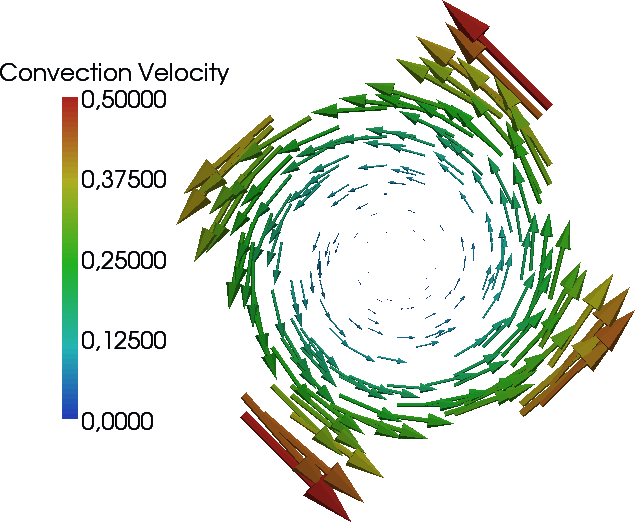
\includegraphics{fig/convection_velocity.png}}
\caption{Convection velocity $a$ for the instationary problem}
\label{convectinvelocity}
\end{center}
\end{figure}

\subsection{$\theta$-Family of Time Discretization Methods}

For the explicit Euler method \index{Euler!explicit} we tested with $\Delta t = 1$ on a six times refined grid, see Figure \ref{explicit}.

\begin{figure}[htbp]
\begin{center}
\scalebox{0.45}{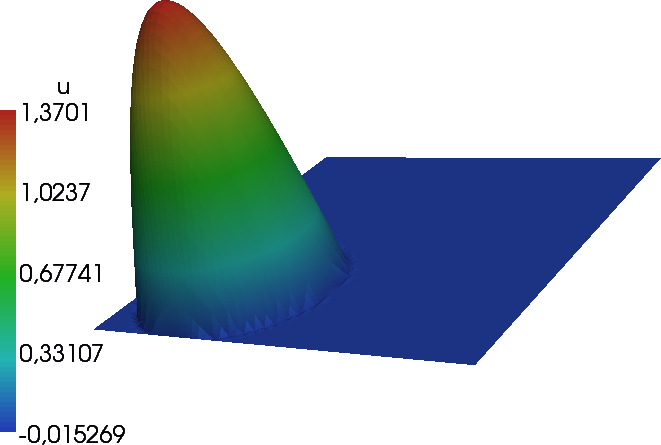
\includegraphics{fig/explicit_ref6_step1.png}}
\caption{Solution at $T = 100$ computed by explicit Euler for $\Delta t = 1$ on a six times refined grid}
\label{explicit}
\end{center}
\end{figure}

As we can see the source is not transported, because the method is of too low order, even though it is stable.

For the Crank-Nicolson method\index{Crank-Nicolson} we started with the same setting, see Figure \ref{crank_ref6_step1}. As we can see, the solution is stable and we get the expected helical solution.

\begin{figure}[htbp]
\begin{center}
\scalebox{0.45}{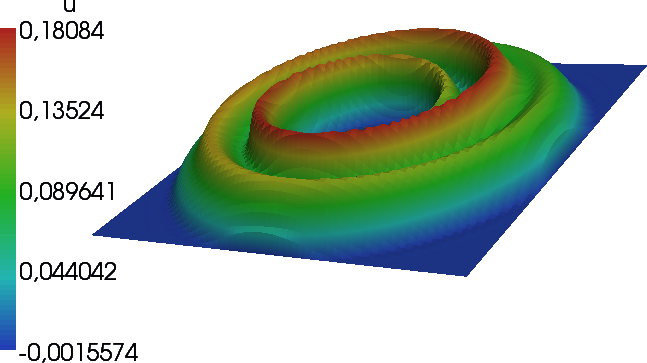
\includegraphics{fig/crank_ref6_step1.png}}
\caption{Solution at $T = 100$ computed by Crank-Nicolson for $\Delta t = 1$ on a six times refined grid}
\label{crank_ref6_step1}
\end{center}
\end{figure}

But the big time-step size leads to a solution that is too diffusive. Repeating the same test case with different time-step sizes and levels of refinement shows that the "waves" should be more distinctive, see Figures \ref{crank_ref6_step0.1} and \ref{crank_ref8_step0.1}.

\begin{figure}[htbp]
\begin{center}
\scalebox{0.35}{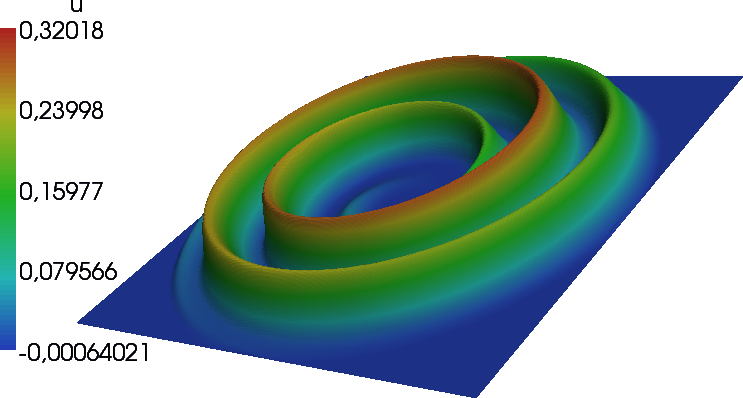
\includegraphics{fig/crank_ref8_step0,2.png}}
\caption{Solution at $T = 100$ computed by Crank-Nicolson for $\Delta t = 0.2$ on a eight times refined grid}
\label{crank_ref6_step0.1}
\end{center}
\end{figure}

\begin{figure}[htbp]
\begin{center}
\scalebox{0.35}{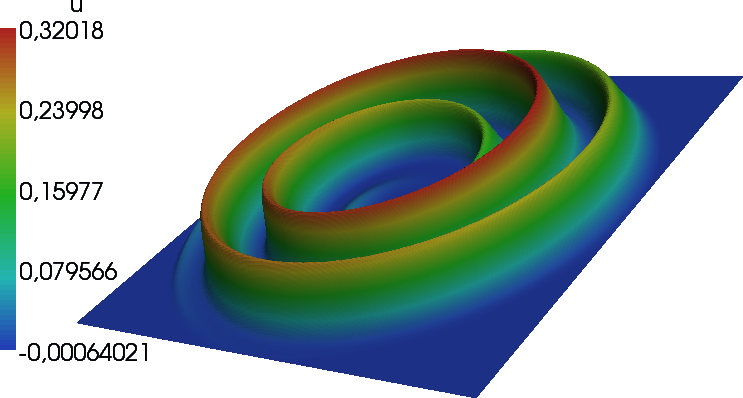
\includegraphics{fig/crank_ref8_step0,1.png}}
\caption{Solution at $T = 100$ computed by Crank-Nicolson for $\Delta t = 0.1$ on a eight times refined grid}
\label{crank_ref8_step0.1}
\end{center}
\end{figure}

For the implicit Euler method\index{Euler!implcit} we ran the same tests as for the Crank-Nicolson method except for the test on refinement level eight, see Figures \ref{implicit_ref6_step1} and \ref{implicit_ref6_step0.1}.

\begin{figure}[htbp]
\begin{center}
\scalebox{0.45}{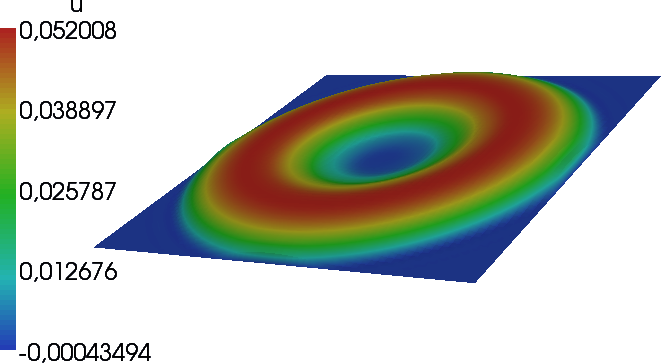
\includegraphics{fig/implicit_ref6_step1.png}}
\caption{Solution at $T = 100$ computed by implicit Euler for $\Delta t = 1$ on a six times refined grid}
\label{implicit_ref6_step1}
\end{center}
\end{figure}

\begin{figure}[htbp]
\begin{center}
\scalebox{0.35}{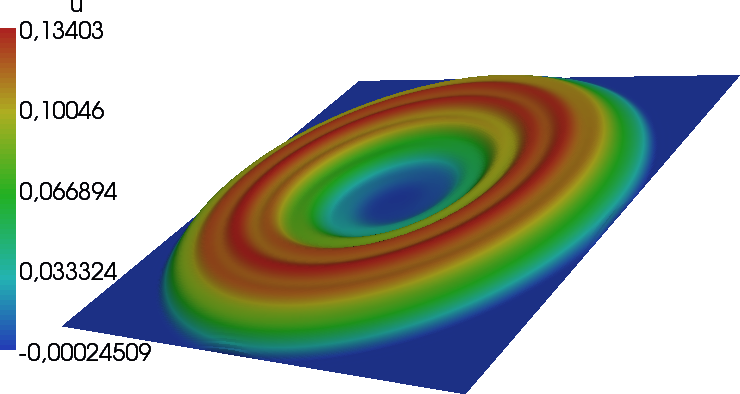
\includegraphics{fig/implicit_8_step0,1.png}}
\caption{Solution at $T = 100$ computed by implicit Euler for $\Delta t = 0.1$ on a eight times refined grid}
\label{implicit_ref6_step0.1}
\end{center}
\end{figure}

This method is even more diffusive than the Crank-Nicolson, but also a bit more stable. The advantage of Crank-Nicolson is that it is compared with the explicit and implicit Euler methods of second order instead of first order only.

So the Crank-Nicolson method provides the best mixture of stability and quality of the computed solution.

\subsection{The classical Runge-Kutta method}

This method turned out to be stable for time-step sizes smaller than or equal to $\Delta t = 0.015$. As figure \ref{rk_ref6_step0.01} shows the scheme is also too diffusive. Although it is of fourth order it does not provide the accuracy of the Crank-Nicholson scheme, see below.

\begin{figure}[htbp]
\begin{center}
\scalebox{0.3}{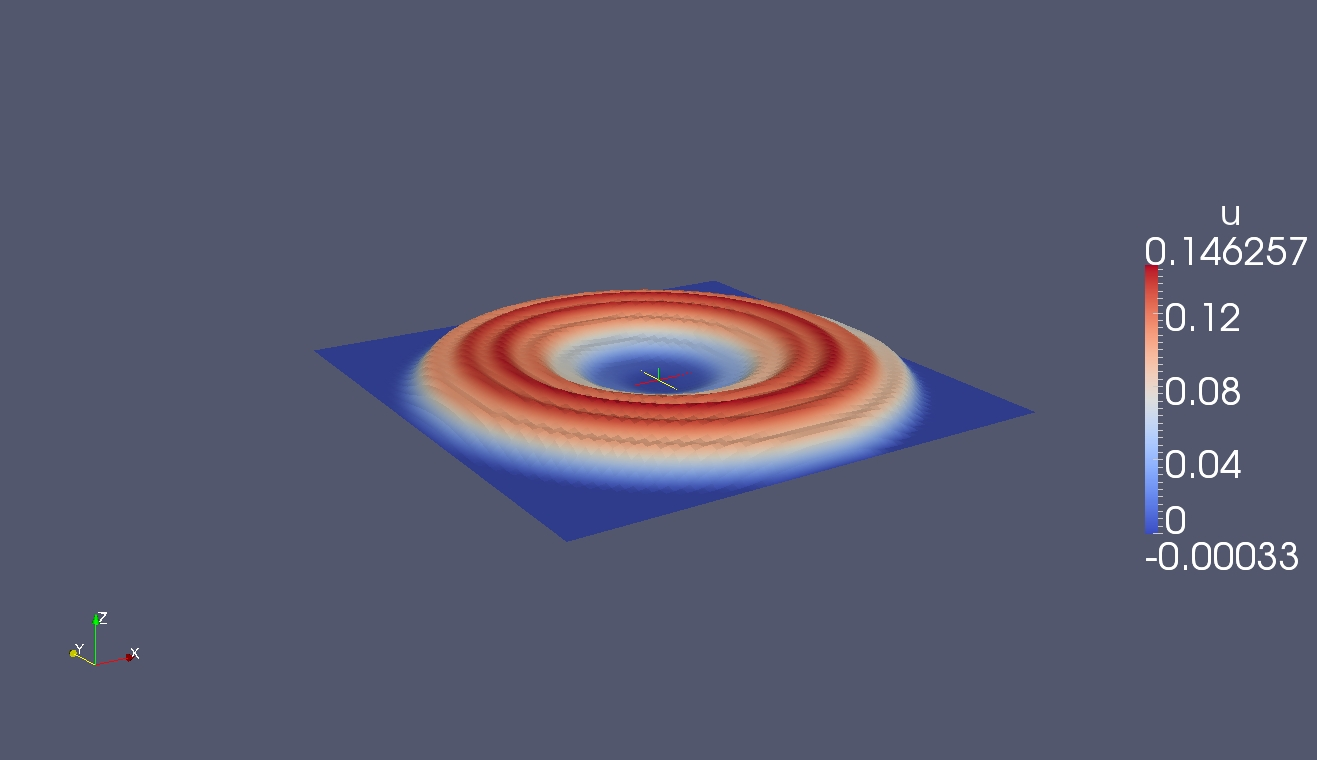
\includegraphics{fig/rk_ref6_step0,01.jpg}}
\caption{Solution at $T = 100$ computed by the classical Runge-Kutta method for $\Delta t = 0.01$ on a six times refined grid}
\label{rk_ref6_step0.01}
\end{center}
\end{figure}

\subsection{Comparison of the two methods}

If we compare the $\theta$ family of methods with the classical Runge-Kutta method we obtain an ambivalent result.

On the one hand the classical Runge-Kutta method is an explicit method which means that one time-step can be computed very fast. One can also use the CG method to compute the $k_{i}$, $i = 1, \ldots, 4$, appearing in the scheme instead of the GMRES solver which is needed for the $\theta$ family. Another advantage of the classical Runge-Kutta method is that it is of fourth order instead of order one (explicit and implicit Euler) or order two (Crank-Nicholson).

On the other hand the classical Runge-Kutta methods needs significantly smaller time-step sizes than e.g. the Crank-Nicholson or implicit Euler scheme. This cirumstance not only leads to longer computation times but in particular the amount of rounding errors is potentially increased. That way the classical Runge-Kutta method looses its fourth-order-advantage compared to the Crank-Nicholson scheme although the latter is of second order only.

In summary we recommend to use the Crank-Nicholson time-stepping scheme because it provides the best compromise between stability and accuracy of the solution.


\newpage
\appendix
\bibliography{tutorials_bib}
\bibliographystyle{plain}

\printindex

\end{document}
